\documentclass[11pt]{article}
\usepackage[margin=1in]{geometry}
\usepackage{amsmath, amssymb, amsthm, enumerate}
\usepackage{graphicx,url, hyperref,framed, esint, color, tikz}

\setcounter{secnumdepth}{-2}

\begin{document}
\begin{flushright}
Alex Rich and Aaron Rosen\\
Engineering 155 \\ 
Final Project Proposal\\
November 16, 2015
\end{flushright}
\section{Final Project Proposal: A Robot Controlled Over The Internet}
The team proposes to build a robotic vehicle that takes inputs from a website as commands and executes them.  The website is to be hosted from an E155 Raspberry Pi2 Apache2 server, and will contain a visual grid interface.  The user will click on different points on the grid to input commands into a list to be sent to the vehicle upon clicking a submission button.  The Pi will parse the commands and send them using a BlueSMiRF to another BlueSMiRF on the vehicle.  The vehicle�s controller (the E155 $\mu$Mudd board) will read these commands and execute them. Below we will go over the deliverables for each part (website, Pi, FPGA, vehicle, new hardware) in detail.

\subsection{Website}
The website will contain a visual UI that contains instructions for use, a grid on which to input locations for the robot to maneuver to, a list of the locations currently buffered for sending, a �clear buffer�, and a submission button, which submits the commands to the Pi for communication.  

%Stretch goals include control for any vehicle peripherals in the event that the stretch goal for the vehicle is complete.

\subsection{Raspberry Pi 2}
The Pi will be providing a server to host the website.  It will connect to a BlueSMiRF with a Bluetooth dongle in order to transmit data to the vehicle.  Upon receiving the list of locations from the website, the Pi will send one command at a time (waiting for ACK of successful execution from the vehicle).

\subsection{FPGA}
The FPGA will connect to a BlueSMiRF over UART.  The UART will be implemented by the team.  The FPGA will execute the command received by controlling the two motors via the H-Bridges on the $\mu$Mudd board.  

%Stretch goals include control of the vehicle peripheral in the event that the stretch goal for the vehicle is complete.

\subsection{Vehicle}
The vehicle will have two motors, one that controls each tank tread.  The motors will be wired to the H-Bridges.  The chassis will be purchased, and the motors will be sourced from the Engineering Department (E11 motor package) if possible.  

%The stretch goal is to implement a peripheral device (e.g. a tank cannon, bulldozer blade, excavator shovel, etc.) that can be controlled from the website.

\subsection{New Hardware}
The new hardware for the project is a BlueSMiRF that will allow for communication between the Pi and the FPGA.  The device communicates with other devices using UART hardware and communicates with other BlueSMiRFs using Bluetooth.

\subsection{Overview of System}
A diagram of our system is shown below. The system is comprised of two major subsystems: the Raspberry Pi 2 controller and the vehicle, which is controlled by the $\mu$Mudd board.
\begin{center}
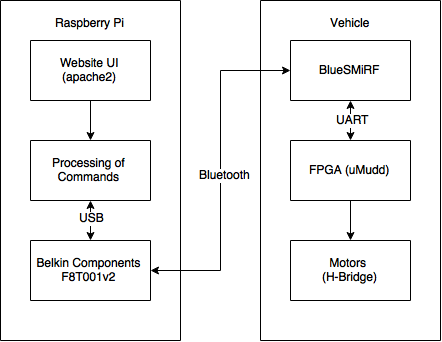
\includegraphics[width=0.9\textwidth]{E155System}
\end{center}

\section{Bill of Materials}

\centering
\begin{tabular}{|l|l|l|l|}
\hline
\multicolumn{1}{|c|}{\textbf{Item}} & \multicolumn{1}{c|}{\textbf{Description}}               	& \multicolumn{1}{c|}{\textbf{Source}} & \multicolumn{1}{c|}{\textbf{Cost}} \\ \hline
Tracked Vehicle 			&										&							&	\\
			Chassis Kit	& Chassis for the tank, includes treads and frame.    	& Amazon 					& 15.39                          	\\ \hline
Tamiya 70168				& Gives tank flexibility to turn by controlling each     	& 							& \\
Double Gearbox			& tread independently.						& Amazon		               			& 11.99                             	\\ \hline
$\mu$Mudd Board                	& Controls the vehicle                                                 & E155                                 		& 0.00                               	\\ \hline
			                      	& Provides website interface and sends commands 	&							&\\
Raspberry Pi 2			    	& to vehicle             							& E155                                 		& 0.00                               	\\ \hline
                        				& Wirelessly communicate via Bluetooth between  	&							&\\
2X BlueSMiRF				& Pi and $\mu$Mudd board. 					& E155                                		& 0.00                               	\\ \hline
2X TrustFire 14500			& Li Ion battery, 3.7 V 						& Aaron Rosen					& 0.00				\\ \hline
\end{tabular}

\end{document}


























